\documentclass[a4paper,10pt]{article}
\usepackage[utf8]{inputenc}
\usepackage[pdftex]{graphicx}
\usepackage{caption}
\usepackage{subcaption}
\usepackage{verbatim}

%opening
\title{Filtro Digital IIR utilizando aproximação Elíptica}
\author{Danilo Souza, Hugo Santos, Welton Araújo}

\begin{document}

\maketitle

\section{Introdução}
%Existe uma necessidade muito grande em processamento de sinais em tratar sinais de entrada em uma determinada banda de frequência. Isto só é possível por meio de uma função de transferência com uma razão de polinômios para gerar filtros com resposta ao impulso de duração infinita(IIR).

%Filtros IIR têm uma melhor aplicação prática por conta de precisar de menos multiplicações para realizar uma aproximação. Diferentemente de filtros com resposta ao impulso finitas(FIR), pois possuem mais dificuldade na atuação em processamento de sinais em tempo real.

%O método de aproximação adotado neste trabalho, o elíptico, tem sua origem no domínio do tempo contínuo. Por conseguinte, é necessária uma transformação para o tempo discreto, através da transformação bilinear.

Devido à grande dificuldade para se trabalhar com sinais reais, em função da grande  presença de rúido existente no universo analógio, a utilização de filtros é de fundamental importância para processamento digital de sinais, atuando na eliminção de ruído indesejado, preservando assim o sinal de interesse. Esta operação é feita no domínio da frequência, onde o filtro possui uma resposta representada por magnitude e fase, uma vez que a saída de um Sistema Linear e Invariante no tempo é dada pela convolução da entrada com a resposta ao impulso do sistema, que, no domínio da frequência, corresponde à multiplicação da Resposta em Frequência pela transformada de Fourier do sinal de entrada.

A fase da Resposta em Frequência indica a defasagem do sinal com relação ao sinal de entrada do sistema de filtragem e a resposta em magnitude representa as bandas de passagem, de corte e de transição, sendo esta última um ponto chave no projeto de filtros, uma vez que, dependo da aplicação, pode ser crucial ter uma banda de transição pequena, enquanto que em outros casos não é necessária uma grande rigidez para essa faixa de frequências do espectro.
 
Os filtros digitais são divididos em duas categorias, FIR (Resposta ao Impulso Infinita) e IIR (Resposta ao Impulso Infinita), sendo esta última apenas o mapeamento de filtros analógicos amplamente conhecidos e estudados, como Filtro de Chebyshev, Butterworth e Elíptico (Cauer), para o universo digital. 
Este trabalho tem por objetivo mostrar uma implementação do filtro Elípitco, usando o MatLab, tomando como referência dois filtros, um passa-baixa e outro rejeita-faixa, descritos abaixo:   



Uma das grandes vantagens de se trabalhar com filtros IIR é que quando comparados com filtros FIR com os mesmos requisitos de projeto, apresentam menor ordem, por este motivo precisam realizar menos multiplicações, diminuindo assim os recursos para implementação, entretanto por apresentarem resposta ao impulso infinita possuem um problema com a estabilidade, para garantir um filtro estável o projeto deve ser feito de tal forma que os pólos da Função de Transferência  sejam internos ao círculo de raio unitário do plano Z. Outro problema dos filtros IIR é que não há controle sobre a fase da Resposta em Frquência, os filtros são projetados levando em consideração somente a magnitude, portanto não sendo indicados para aplicações que necessitam de filtros com fase linear (p.e. processamento de imagem).

Algumas vantagens e desvantagens de se trabalhar com filtros elíptcios são listadas abaixo:
%Uma vantagem em particular do filtro Elíptcio quando comparado com outros filtros IIR é que possui um declive mais acentuado na banda de transição, o que o torna mais adequado para aplicações que necessitam de uma maior rigidez em relação à banda de transição. Embora possuam a menor ordem dentre os filtros IIR, os filtros elípticos são considerados mais difíceis de projetar.

\subsection{Vantagens}

	\begin{itemize}
		\item Menor ordem quando comparados com filtros FIR
		\item Maior declive na curva de transição
	\end{itemize}


\subsection{Desvantagens}

	\begin{itemize}
		\item Não possuem fase linear
		\item Resposta ao impulso infinita (Estabilidade)
		\item Sâo difíceis de projetar e analisar
	\end{itemize}


Existem basicamente duas abordagens para projetar um filtro Elíptico:

\subsection{Abordagens para construção de Filtros Elípticos}
	\subsubsection{Abordagem I}
	
		\begin{itemize}
			\item Projetar filtro Passa-Baixa analógico
			\item Realizar transformação em frequência (s \(\rightarrow\) s)
			\item Aplicar transformação do filtro (s \(\rightarrow\) z)
		\end{itemize}

	\subsubsection{Abordagem II}
		\begin{itemize}
			\item Projetar filtro Passa-Baixa analógico.
		\end{itemize}
		\begin{itemize}
			\item Aplicar transformação do filtro (s $\rightarrow$ z).	
		\end{itemize}	
		\begin{itemize}
			\item Realizar transformação em frequência (z $\rightarrow$ z).
		\end{itemize}	
	
	
	A transformação do filtro do plano \textit{s} para o plano \textit{z} pode ser feita usando dois métodos, invariância da resposta ao impulso e transformação bilinear, sendo este úlitmo, o método utilizado neste trabalho, juntamente com a Abordagem I.
	
\section{Projetos dos Filtros}

\subsection{Achar a frequência digital \(\omega\) para posterior distorção de frequências analógicas}
	O início do projeto de um filtro se define em calcular as frequências digitais equivalentes às frequências analógicas indicadas pelos requisitos dos filtros desejado, a forma de calcular está apresentada em \eqref{(1)}
	
	\begin{equation}\label{(1)}
		\omega = \frac{2\pi \Omega}{\Omega_{s}}
	\end{equation}	
	
	Uma vez calculadas as frequências digitais, é necessário calcular as frequências analógicas distorcidas que serão usadas para encontrar os coeficientes do filtro normalizado, o cálculo destas frequências é mostrado na equação \eqref{(2)}

\subsection{Frequências distorcidas \Omega}

	\begin{equation}\label{(2)}
		\Omega = \frac{2}{T}\tan\frac{\omega}{2}
	\end{equation}
	Com estes resultados é possivel calcular as frequências normalizadas do filtro passa-baixa normalizado. As equações (5) e (6) mostram como calcular a constante de transformação \textit{a} para filtros passa-baixa e filtros rejeita-faixa respectivamente.
	
\subsection{Definindo algumas constantes para calcular a ordem do filtro}
	
	
	\begin{equation}
		a = \Omega_{r}'
	\end{equation}
	\begin{equation}
		a = \frac{1}{\Omega_{p}'}
	\end{equation}
	
	\begin{equation}\label{valor de \textit{a} para filtros passa-baixa}
		a = \sqrt{\frac{\Omega_r}{\Omega_p}}
	\end{equation}
	
	\begin{equation}\label{valor de \textit{a} para filtros rejeita-faixa}
		a = \sqrt{\frac{\Omega_{p2} - \Omega_{p1}}{\Omega_{r2} - \Omega_{r1}}}	
	\end{equation}
	
	\begin{equation}
		k = \frac{1}{\Omega_r^{2}'}
	\end{equation}
	\begin{equation}
		q0 = {\frac{1}{2} \frac{1-(\sqrt[4]{1-k^{2}}}{1+(\sqrt[4]{1-k^{2}}}}
	\end{equation}
	\begin{equation}
		q = q0 + 2q0^{5} + 15q0^{9} + 150qo^{13} 
	\end{equation}
	\begin{equation}
		e = \sqrt{\frac{10^{0.1ap}-1}{10^{0.1ar}-1}}
	\end{equation}
	\begin{equation}
		n \geq \frac{\log_{10}\frac{16}{e^{2}}}{\log_{10}\frac{1}{q}}
	\end{equation}
	
	Após o cálculo da ordem n do filtro, é necessário calcular mais alguns parâmetros para que ao final do processo seja possível encontrar os coeficientes do filtro normalizado

	\begin{equation}
		\Theta\ = \frac{1}{2n}ln\frac{10^{0.05A_{p}} + 1}{10^{0.05A_{p}} - 1}
	\end{equation}
	
	\begin{equation}
		\sigma\ =  \frac{2q^{\frac{1}{4}}\sum_{j=0}^{\infty} (-1)^{j} q^{j(j+1)} senh[(2j+1)\Theta]}								{1+2\sum_{j=1}^{\infty}  (-1)^{j} q^{j^{2}} cosh[(2j\Theta]}
	\end{equation}
	
	\begin{equation}
		W = \sqrt{(1+k\sigma^{2})(1+\frac{\sigma^{2}}{k})}
	\end{equation}
	\begin{equation}
		\Omega_{i}' =	\frac{2q^{\frac{1}{4}}\sum_{j=0}^{\infty} (-1)^{j} q^{j(j+1)} sen(\frac{(2j+1)\pi 		u}		{n})}								{1+2\sum_{j=1}^{\infty}  (-1)^{j} q^{j^{2}} 					cos(\frac{2j\pi u}			{n})}
	\end{equation}
	\begin{equation}
		V_{i} = \sqrt{(1-k\Omega_{i}^{2}')(1-\frac{\Omega_{i}^{2}'}{k})} ,
	\end{equation}
	
	onde
	
	\begin{itemize}
		\item \textit{u} = \textit{i},  para \textit{n} ímpar
		\item \textit{u} = \textit{i}-1/2,  para \textit{n} par	
	\end{itemize}
	
	\begin{equation}
		H'(\textit{s}') = \frac{H'_{0}}{(\textit{s}'+\sigma^{m})} \prod_{i=1}^{l} \frac {\textit{s}'^{2} 																						+b_{2i}}														{\textit{s'^{2}}+\textit{a}_{li}\textit{s}'+\textit{a}_{2i}},
	\end{equation}
		onde 
		
		\begin{itemize}
			\item {m = 0 e l = \frac{n}{2},
			 para \textit{n} par}
			
			\item {m = 1 e l = \frac{\textit{n}-1}{2},
			 para \textit{n} ímpar}
		\end{itemize}
		\begin{equation}
			b_{2i} = \frac{1}{\Omega'^{2}_{i}}
		\end{equation}
		\begin{equation}
			a_{2i} = \frac{(\sigma V_i)^{2} + (\Omega'_{i}W)^{2}}{(1+\sigma^{2}\Omega'^{2}_{i})^{2}}
		\end{equation}
		\begin{equation}
			a_{li} = \frac{2\sigma V_{i}}{(1+\sigma^{2}\Omega'^{2}_{i})}
		\end{equation}		
		\begin{equation}
			H'_{0} = \sigma \prod_{i=1}^{l}\frac{\textit{a}_{2i}}{\textit{b}_{2i}}
		\end{equation} para n ímpar
		\begin{equation}
			H'_{0} = 10^{-0.05A_{p}}\sigma \prod_{i=1}^{l}\frac{\textit{a}_{2i}}{\textit{b}_{2i}}					\end{equation} para n par
			
		A partir da equação (17) e aplicando o resultado das equações (18), (19), (20), (21) ou (22) está completo o cálculo dos coeficientes do filtro normalizado.
		
\subsection{Transformação em Frequência}
	A partir deste ponto precisa-se criar um filtro analógico desnormalizado, essa mudança depende do tipo de filtro. as equações (23) e (24) mostram a desnormalização de passa-baixa para baixa-baixa e de passa-baixa para rejeita-faixa.

	\begin{equation}	
		s' \leftrightarrow \frac{1}{a} \frac{s}{\Omega_{p}}
	\end{equation}
	
	\begin{equation}
		s' \leftrightarrow \frac{1}{a} \frac{B_{s}}{s^{2} + \Omega_{0}^{2}}
	\end{equation}
	
	Após essa transformação, o resultado é a função para se encontrar o filtro digital através da transformação bilinear. 
				
\subsection{Método da Transformação Bilinear}
Consiste no mapeamento da metade esquerda do plano \textit{s} dentro de uma circunferência unitária do plano \textit{z} através de uma normalização do espectro analógico da frequência de um intervalo \(-\infty < \Omega < \infty\) para \(-\pi < \omega < \pi\). 

Sua vantagem se deve ao fato de evitar o \textit{aliasing}, portanto mantém as características do módulo da resposta em frequ\^encia do filtro anal\´ogico para a resposta em frequ\^encia do filtro digital.

O método da transformação bilinear baseia-se na seguinte relação:

	\begin{equation} \label{(1)}
		\[s = \frac{2}{T} \frac{(1-Z^{-1})}{1+Z^{-1}}\]
	\end{equation}
	\begin{equation} \label{(2)}
		\[z = \frac{(1+s(T/2)}{1-s(T/2)}\]
	\end{equation}


Resolvendo esta relação para as frequ\^encias \(\omega\) (digital) e \(\Omega\) (analógica), obtém-se as seguintes relações:

\begin{equation} \label{(3)}
\[\omega = \frac{2\(\arctan(\Omega T)}{2}\]
\end{equation}
\begin{equation} \label{(4)}
\[\Omega = \frac{2}{T}\tan(\frac{\omega }{2})\]
\end{equation}

Para realizar a transformação bilinear é necessário encontrar primeiramente as frequências pré-distorcidas, pois esta transformação resulta em um erro muito grande para altas frequência, por isso a necessidade de achar as frequências distorcidas para todos os casos, para que então a transformação possa ser feita de fato. Essas frequências são encontradas utilizando \eqref{(3)} e/ou \eqref{(4)}


\subsection{Filtro I}
\begin{table}[ht]
\centering
\begin{tabular}{|l|l|}

\(A_p\) 	& 1 dB		\\
\(A_r\) 	& 40 dB		\\
\(\Omega_p\) 	& 1000 Hz	\\
\(\Omega_r\) 	& 1290 Hz	\\
\(\Omega_s\) 	& 3000 Hz	\\

\end{tabular}
\caption{Propriedades do filtro I}
\label{tab:tabfiltro1}
\end{table}

Trata-se de um filtro passa-baixa. Suas especificações estão inseridas na Tabela \ref{tab:tabfiltro1}. Onde \(A_p\) e \(A_r\) são a atenuação máxima e mínima nas frequências de passagem e rejeição, respectivamente e \(\Omega_p\), \(\Omega_r\) e \(\Omega_s\) são as frequências de máxima de passagem, mínima de rejeição e de amostragem, respectivamente.

A equação de diferença gerada por esse filtro é: 
\[0,4229y[n+3] + 0,3303y[n+2] \]
\[ + 0,2635y[n+1] - 0,0151y[n] = 0,1300x[n+3] + 0,3708x[n+2]  \]
\[+ 0,3708x[n+1] + 0,1300x[n]

A expressão da transformada Z é:
\[0,1300z^3 + 0,3708z^2 + 0,3708z^1 + 0,1300 \]
\hline
\[0,4229z^3 + 0,3303^2 + 0,2635z - 0,0151 \]

A expressão da transformada de Fourier é:
\[0,1300e^{jw3} + 0,3708e^{jw2} + 0,3708e^{jw} + 0,1300 \]
\hline
\[0,4229e^{jw3} + 0,330e^{jw2} + 0,2635e^{jw} - 0,0151 \]

\subsection{Filtro II}

\begin{table}[ht]
\centering
\begin{tabular}{|l|l|}

\(A_p\) 	& 0,5 dB	\\
\(A_r\) 	& 60 dB		\\
\(\Omega_p1\) 	& 40 rad/s	\\
\(\Omega_r1\) 	& 50 rad/s	\\
\(\Omega_p2\) 	& 70 rad/s	\\
\(\Omega_r2\) 	& 80 rad/s	\\
\(\Omega_s\) 	& 240 rad/s	\\

\end{tabular}
\caption{Propriedades do filtro II}
\label{tab:tabfiltro2}
\end{table}

Trata-se de um filtro rejeita-faixa. Suas especificações estão inseridas na Tabela \ref{tab:tabfiltro2}. Onde \(A_{p1}\) e \(A_{r1}\) são a atenuação máxima e mínima nas frequências de passagem e rejeição, respectivamente. \(\Omega_{p1}\) e \(\Omega_{r1}\) são as frequências  máxima de passagem e mínima de rejeição, respectivamente, da faixa inicial. \(\Omega_{p2}\), \(\Omega_{r2}\) são as frequências mínima de passagem, máxima de rejeição, respectivamente, da faixa final.
A frequ\^encia de amostragem \'e representada por \(\Omega_s\).

A equação de diferença gerada por esse filtro é: 
\[        3,0689y[n+10] 		- 0,0093y[n+9] 		+ 6,8268y[n+8] 		- 0,0163y[n+7]\]
\[+  7,7621y[n+6] 		- 0,01116y[n+5] 		+ 4,3854y[n+4] 		- 0,0041y[n+3]\]
\[+ 1,3743y[n+2]		- 0,0004y[n+1] 		+ 0,0268y[n] =			   \]			   

\[0,7329x[n+10] 	- 0,0031x[n+9] 		+ 3,6645x[n+8]		- 0,0124x[n+7]\]
\[+  7,3290x[n+6] 		- 0,0186x[n+5] 		+ 7,3290x[n+4]		- 0,0124x[n+3]\]
\[+ 3,6645x[n+2] 		- 0,0031x[n+1] 		+ 0,7329x[n]  			   \]

A expressão da transformada Z é:
\[0,7329z^{10} 	- 0,0031z^9 		+ 3,6645z^8 		- 0,0124z^7\]
\[+  7,3290z^6 		- 0,0186z^5 		+ 7,3290z^4 		- 0,0124z^3\]
\[+ 3,6645z^2 		- 0,0031z^1 		+ 0,7329			   \]
\hline
\[        3,0689z^{10} 		- 0,0093z^9 		+ 6,8262z^8 		- 0,0163z^7\]
\[+  7,7621z^6 		- 0,01116z^5 		+ 4,3854z^4 		- 0,0041z^3\]
\[+ 1,3743^2		- 0,0004z 		+ 0,0268			   \]

A expressão da transformada de Fourier é:
\[0,7329e^{jw10} 	- 0,0031e^{jw9}  		+ 3,6645e^{jw8} 		- 0,0124e^{jw7} \]
\[+  7,3290e^{jw6}		- 0,0186e^{jw5} 		+ 7,3290e^{jw4} 		- 0,0124e^{jw3}\]
\[+ 3,6645e^{jw2} 		- 0,0031e^{jw1} 		+ 0,7329			   \]			       
\hline
\[        3,0689e^{jw10} 		- 0,0093e^{jw9} 		+ 6,8262e^{jw8}		- 0,0163e^{jw7}\]
\[+  7,7621e^{jw6} 		- 0,01116e^{jw5} 		+ 4,3854e^{jw4} 		- 0,0041e^{jw3}\]
\[+ 1,3743e^{jw2}		- 0,0004e^{jw} 		+ 0,0268\]


%\begin{itemize}
% \item Aplicar-se a pré-distorção nas frequências de passagem e rejeição, \(\omega_p\) e \(\omega_r\), respectivamente, específicas do filtro gerando novas frequências pré-distorcidas, \(\Omega_p\) e \(\Omega_r\).
% \item Gerar a função de transferência analógica \(H_a\)(s)
% \item FALTA O RESTO
% \end{itemize}


\section{Implementação no MatLab}

\subsection{Filtro I}

	
Os gráficos das respostas em frequência em magnitude, magnitude normalizada e fase estão nas Figuras \ref{fig:magnitude1} e \ref{fig:fase1}.

\begin{figure}[ht]
 \centering
 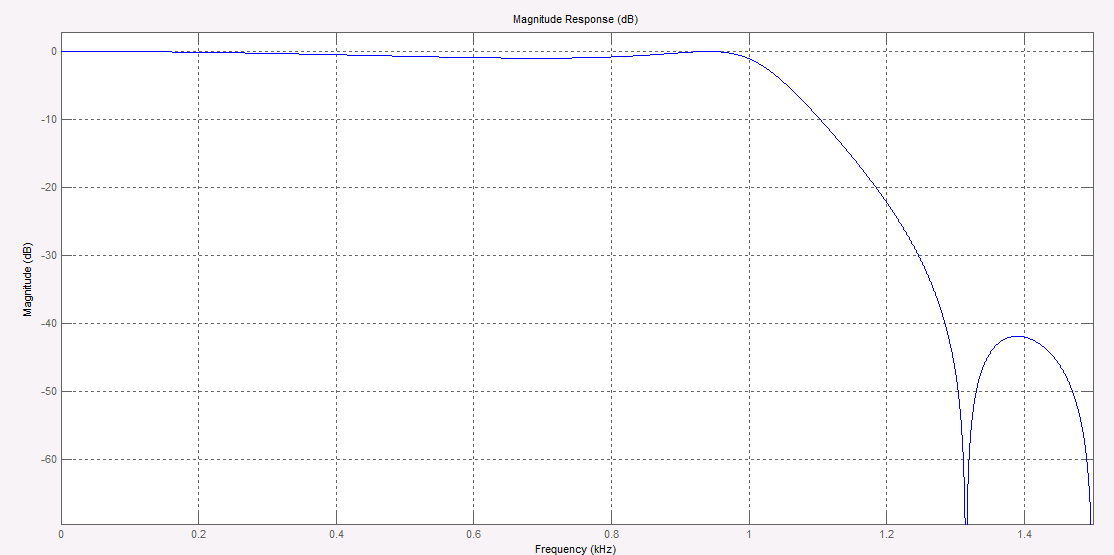
\includegraphics[width=12cm]{pictures/Filtro1/RespMagnitudeFiltro1.png}
 \caption{Resposta em frequência em magnitude do filtro I}
 \label{fig:magnitude1}
\end{figure}

\begin{figure}[ht]
 \centering
 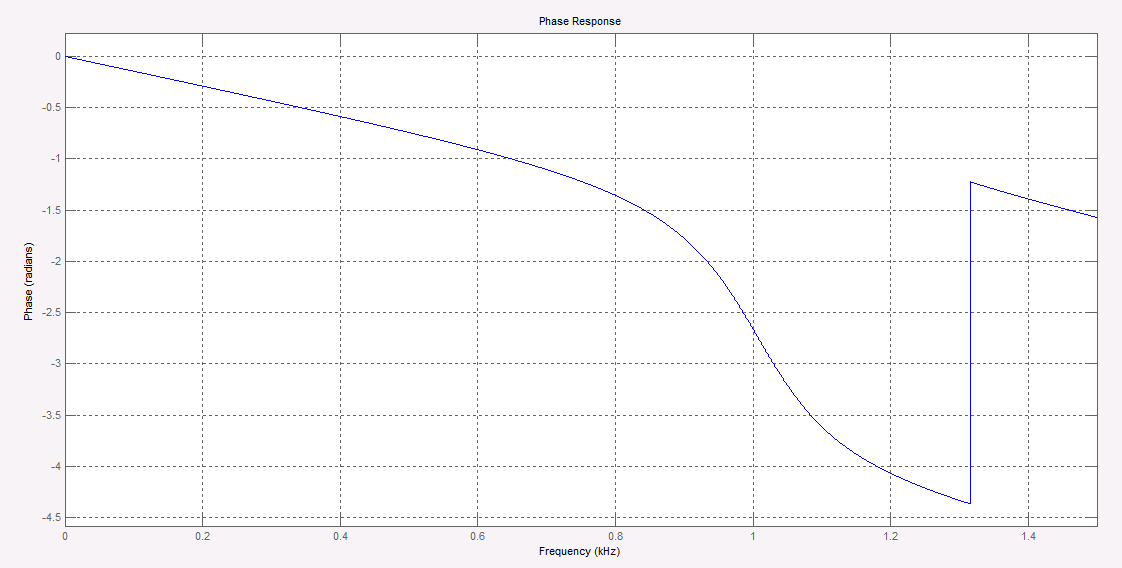
\includegraphics[width=12cm]{pictures/Filtro1/RespFaseFiltro1.png}
 \caption{Resposta em frequência em fase do filtro I}
 \label{fig:fase1}
\end{figure}

O gráfico da resposta ao impulso e o diagrama de polos e zeros estão nas figuras \ref{fig:resimp1} e \ref{fig:diapolozero1}, respectivamente.

\begin{figure}[ht]
 \centering
 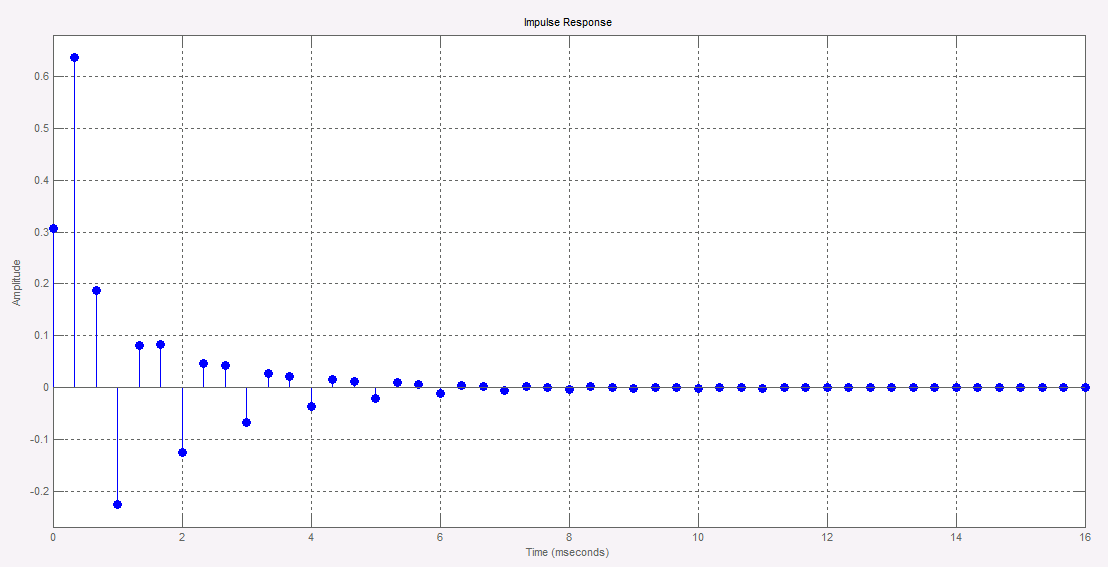
\includegraphics[width=12cm]{pictures/Filtro1/RespImpulsoFiltro1.png}
 \caption{Resposta ao impulso do filtro I}
 \label{fig:resimp1}
\end{figure}

\begin{figure}[ht]
 \centering
 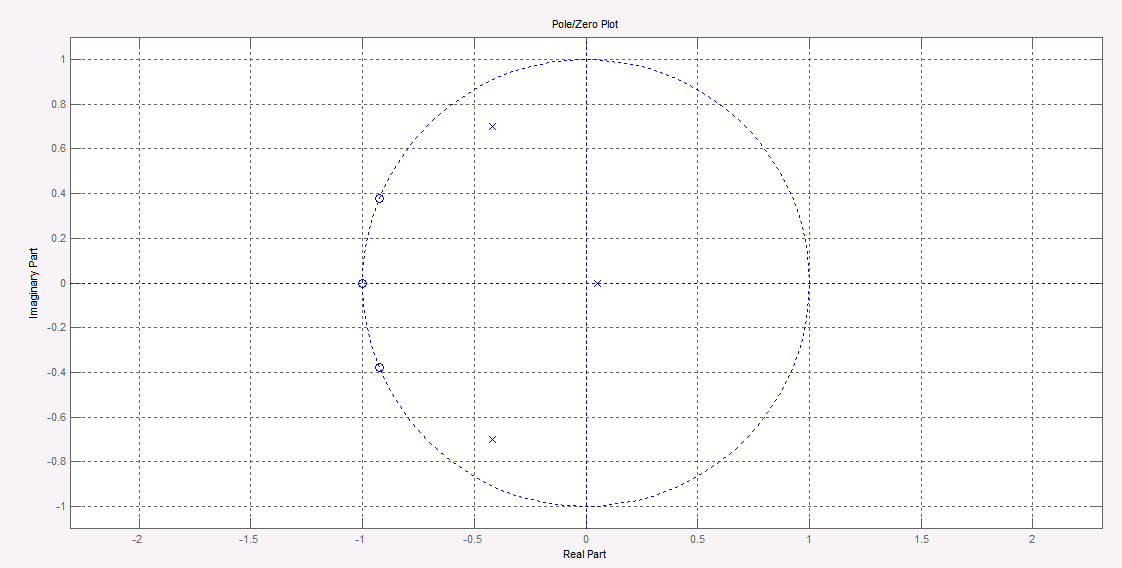
\includegraphics[width=10cm]{pictures/Filtro1/DiagramaFiltro1.png}
 \caption{Diagrama de polos e zeros do filtro I}
 \label{fig:diapolozero1}
\end{figure}

\subsection{Filtro II}

Os gráficos das respostas em frequência em magnitude, magnitude normalizada e fase estão nas Figuras \ref{fig:magnitude2} e \ref{fig:fase2}.

\begin{figure}[ht]
 \centering
 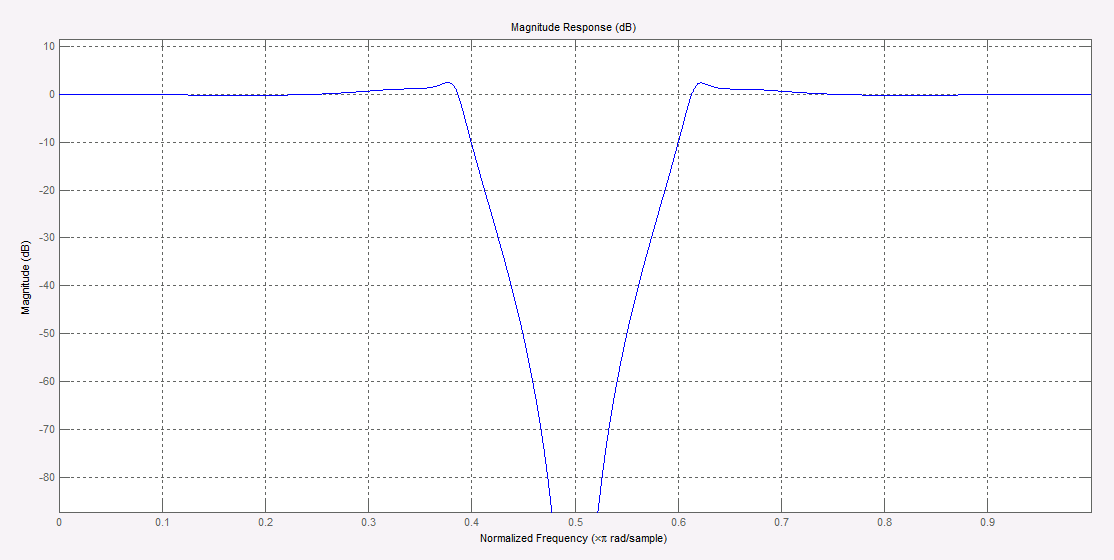
\includegraphics[width=12cm]{pictures/Filtro2/RespMagnitudeFiltro2.png}
 \caption{Resposta em frequência em magnitude do filtro II}
 \label{fig:magnitude2}
\end{figure}

\begin{figure}[ht]
 \centering
 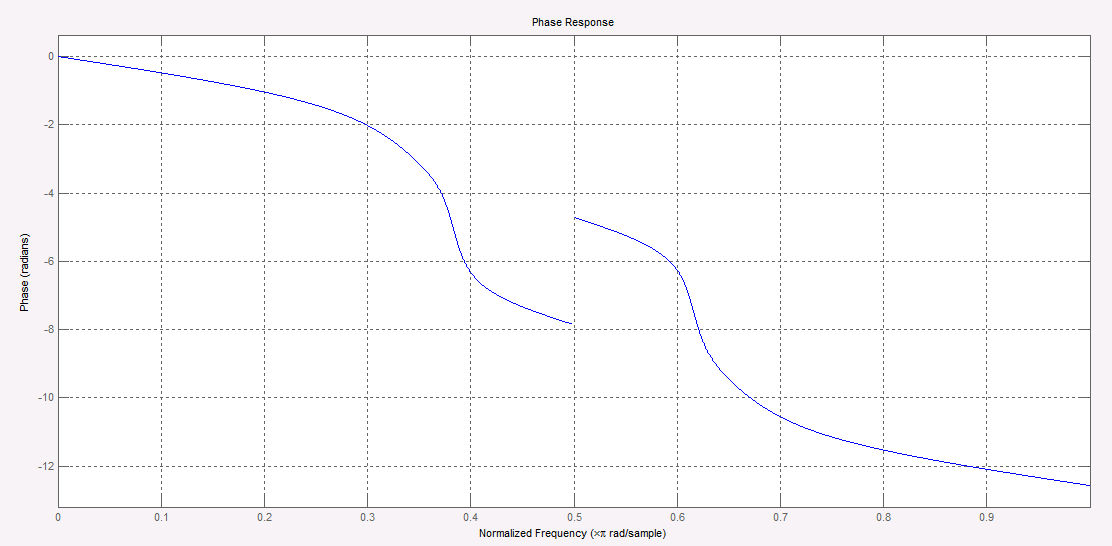
\includegraphics[width=12cm]{pictures/Filtro2/RespFaseFiltro2.png}
 \caption{Resposta em frequência em fase do filtro II}
 \label{fig:fase2}
\end{figure}

O gráfico da resposta ao impulso e o diagrama de polos e zeros estão nas figuras \ref{fig:resimp2} e \ref{fig:diapolozero2}, respectivamente.

\begin{figure}[ht]
 \centering
 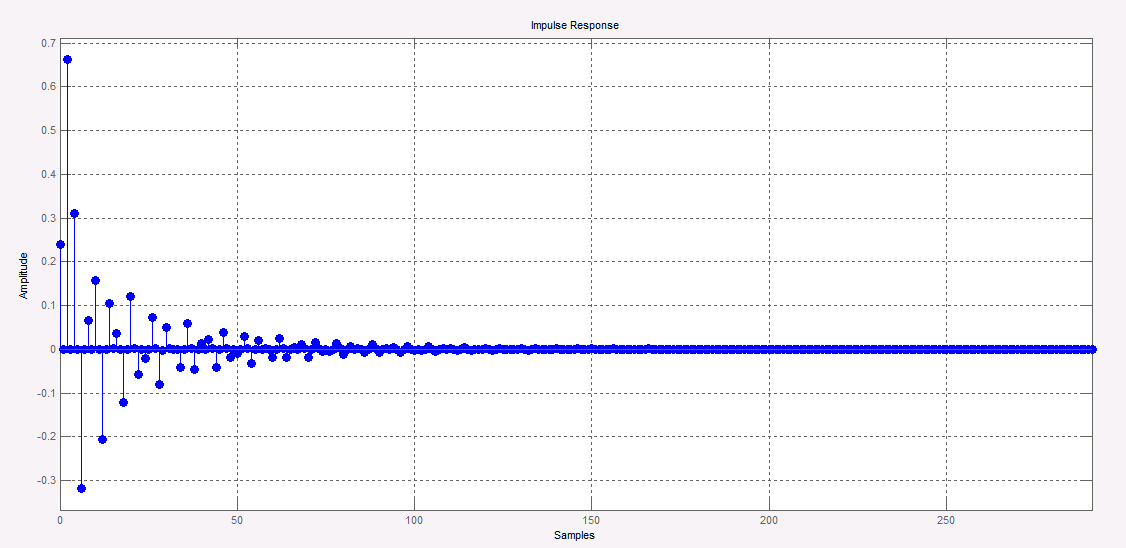
\includegraphics[width=12cm]{pictures/Filtro2/RespImpulsoFiltro2.png}
 \caption{Resposta ao impulso do filtro II}
 \label{fig:resimp2}
\end{figure}

\begin{figure}[ht]
 \centering
 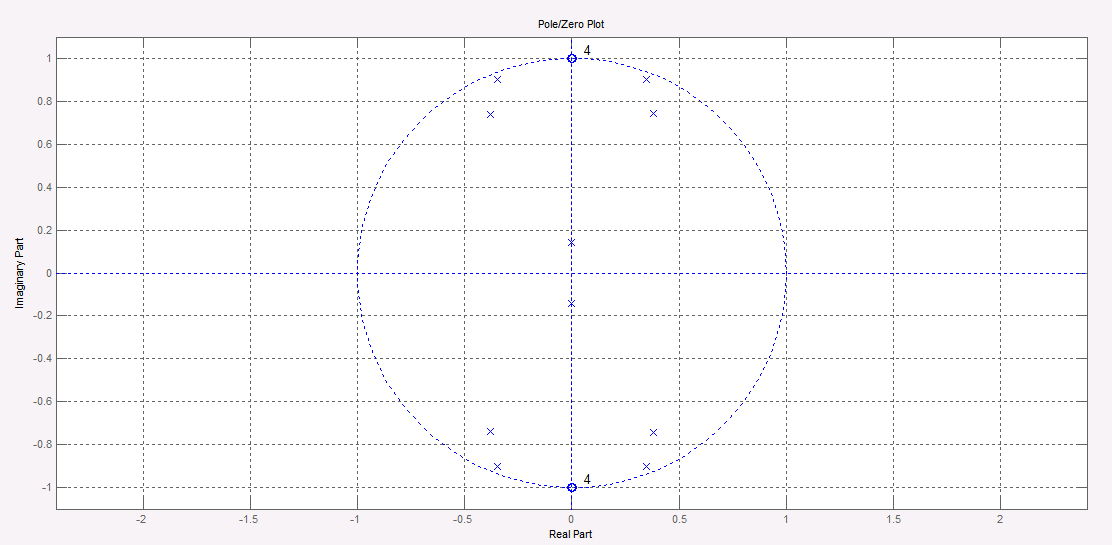
\includegraphics[width=12cm]{pictures/Filtro2/DiagramaFiltro2.png}
 \caption{Diagrama de polos e zeros do filtro II}
 \label{fig:diapolozero2}
\end{figure}

\section{Conclusões}

Com esta implementação, pode-se concluir que filtros IIR com aproximações elípticas possuem um alto grau de complexidade de projeto, pois necessitam de muitas transformações para se obter os coeficientes do filtro desejado. Foi possível confirmar as caracteristicas conhecidas deste tipo de filtro, como Resposta em Fase não linear, \textit{equiripple} nas bandas de passagem e rejeição e um grande declive da Resposta em Frequência na banda de transição. 

AS principais dificuldades no projeto de um filtro elíptico foi a realização dos cálculos nos transformações necessárias, pois essas precisam ser muito precisas e por pequenos erros por parte do grupo, os coeficientes od filtro se diferenciavam do dos coeficientes desejados e por causa deste pequeno desvio o filtro não atendeu de maneira 100\% satisfatória o gabarito do projeto. Isto pode ser comprovado no Filtro II, que possui resultados bem próximos do gabarito, além de ser um filtro estável. Já no Filtro I, o grupo conseguiu superar essas dificuldades, e o resultado do filtro atendeu o gabarito requisitado.

\end{document}
